\section{Pricing Model}
\label{sec:pricing}

%Following the definition of basic concepts in the ride-sharing system, we introduce a general price model that can be utilized to compute the final fare of a rider, the payment drivers receive and subsequently, the profit the ride sharing system generates. Before we continue, it is necessary to point out that one of the building blocks of any real-world ride sharing system is a mechanism for computing the shortest path between any two points in the road network. Without loss of generality, we define our pricing model based on a static shortest path computations as opposed to time-dependent. However, the definitions can be easily updated to be compatible with time-dependent networks as well. For example, the fare of a ride is dependent on the distance between the pick-up and the drop-off points in a static network where in a time-dependent network it can be dependent on the travel time between those two points or perhaps both distance and travel time.

In a ride-sharing platform where the objective is to maximize the monetary profit, it is important to utilize a pricing model which is \textit{fair} to both riders and drivers. For example, with the pricing model introduced in \cref{Ma13}, drivers are compensated based on the distance they have traveled and this is the total fare all riders have to pay. Therefore, for the portions of the trip where there are more than one rider, the fare gets divided by the number of riders on the vehicle. Although it is true that on average, riders are paying less as compared to when riders to not participate in ride-sharing. However, in a simple test on New York City's taxi dateset, we noticed up to 10\% of riders, end up paying even more than what they would have paid if they did not participate in ride-sharing.

In this section we define a generic pricing model which is fair to every user \TODO{mohammad}{make sure in the intro we say what we mean by users} of the system. Before we continue, it is necessary to point out that one of the building blocks of any real-world ride sharing system is a mechanism for computing the shortest path between any two points in the road network. Without loss of generality, we define our pricing model based on a static shortest path computations as opposed to time-dependent. However, the definitions can be easily updated to be compatible with time-dependent networks as well. For example, the fare of a ride is dependent on the distance between the pick-up and the drop-off points in a static network where in a time-dependent network it can be dependent on the travel time between those two points or perhaps both distance and travel time. A fair pricing model has to satisfy the following rules:

\begin{itemize}
\item For \textit{every single rider}, if the rider's trip is longer than the shortest trip between its pick-up and drop-off location, the rider should receive a discount proportional to its trip's detour (i.e., the difference between its actual trip and the shortest trip).
\item For \textit{every single driver}, if the driver's trip is increased for servicing more riders, the driver's compensation should increase proportionate to the distance of the driver's trip.
\end{itemize}

Consequently, every pricing model should define three key concepts: (1) \itqoutes{How much should the riders pay for a trip?} (2) \itqoutes{How much should the drivers make for servicing riders?} and (3) \itqoutes{What is the revenue of the ride-sharing platform?}. Following we define our generic pricing model by answering these three questions.

\subsection{Rider's Fare}

Every request $r$ has a default fare based on the shortest distance, $d_r$, from $r.s$ to $r.e$. In other words, every pricing model should have an arbitrary function $FARE: d \rightarrow \$ $ such that $FARE(d)$ is the default fare of a ride. In a ride-sharing system, the actual route between the pick-up and drop-off locations of a ride is not necessary the shortest route between the two points. We show the actual route between the two end points of a ride with $d'_r$ and define the detour of a ride as $\delta d_r = d'_r - d_r$. As explained in \cref{def:req}, each request is associated with a profile. We introduce the concept of a \textit{rider's profile} as a tool for the rider to specify how much discount she expects to receive in return for a certain amount of detour on her trip. A rider's profile can have different formats: linear decay, exponential decay, etc. \cref{fig:rider_profile} shows an example of a rider's profile.

\begin{figure}[!ht]
	\centering
	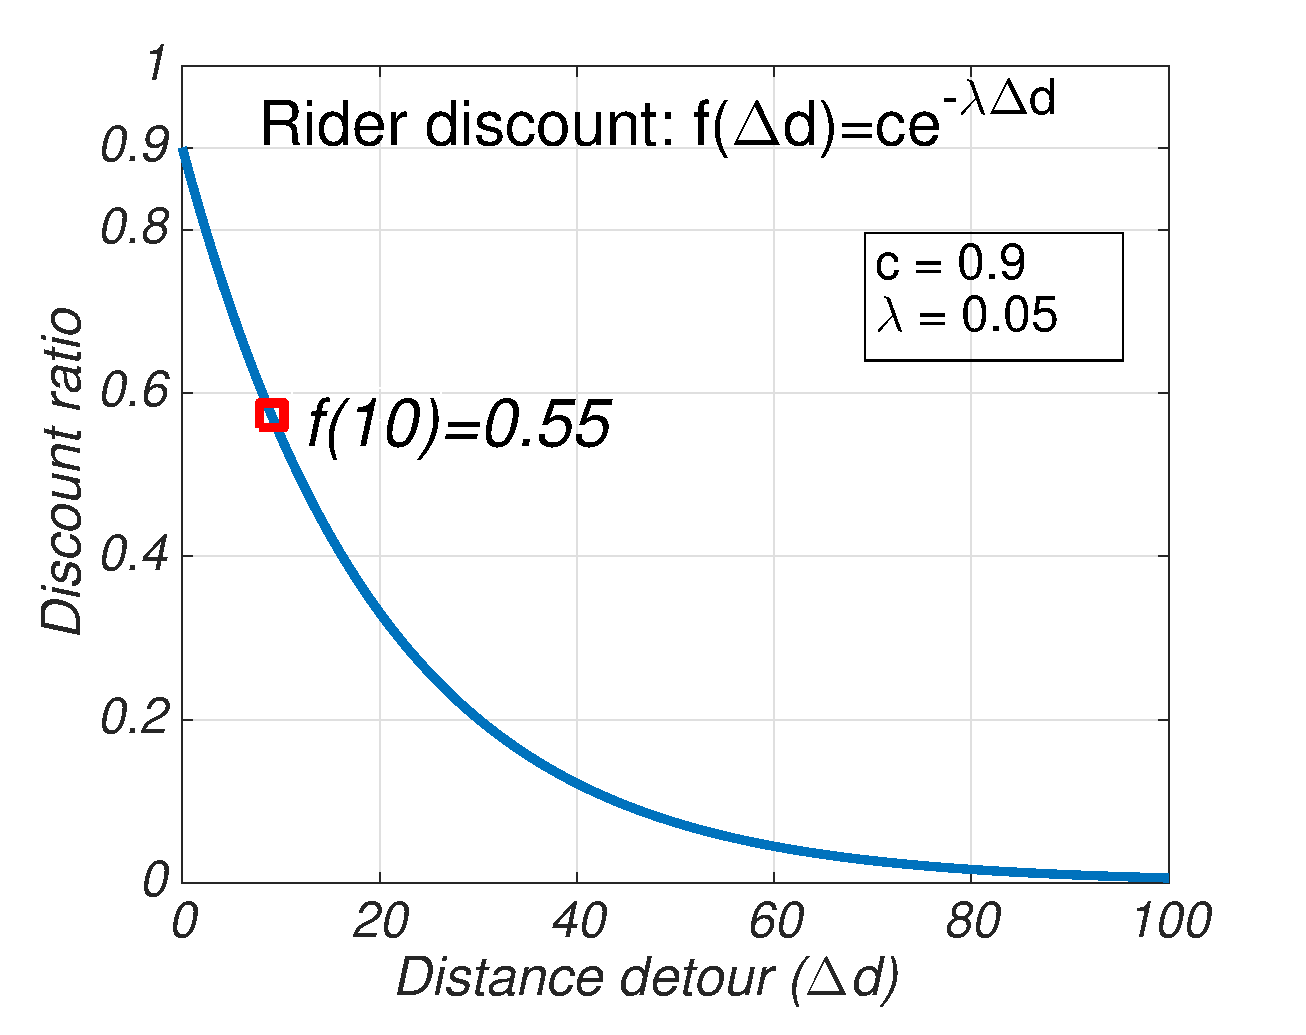
\includegraphics[width = 60mm]{fig/rider.eps}
	\vspace{-0mm}\caption{Rider profile} \vspace{-2mm} \label{fig:rider_profile}
\end{figure}\vspace{-0mm}

Subsequently, for a request $r$ with shortest distance $d_r$, detour $\delta d_r$ and a profile $f_r$, the final fare is:

\begin{equation}
\label{eq:fare}
fare(r) = F(d_r) f_r(\delta d_r)
\end{equation}

This guarantees that no rider can pay more that what he would have payed if he did not participate in ride-sharing. In fact, the rider will get compensated for longer trips based on the detour. This satisfies the first rule of a fair pricing model. 

\subsection{Driver's Income}

Every driver has a unique profile which allows him to specify the cost of his service. Similar to riders, drivers can have different expectations for participating in a ride-sharing platforms. The driver's profile allows each driver to set their expectations with respect to how much they expect to make for participating in the platform. The driver's profile can be any function. In fact, it can take any arbitrary input in addition to the distance. For example, it is possible to define the driver's profile as $g: n, d \rightarrow \$$ where $n$ is the number of passengers being serviced by the driver. Without loss of generality, we assume distance is the only input of the driver's profile. Intuitively, the profile is a monotonically increasing function. For example, the profile in \cref{fig:driver_profile} is one where the driver charges \$1 per mile.

\begin{figure}[!ht]
	\centering
	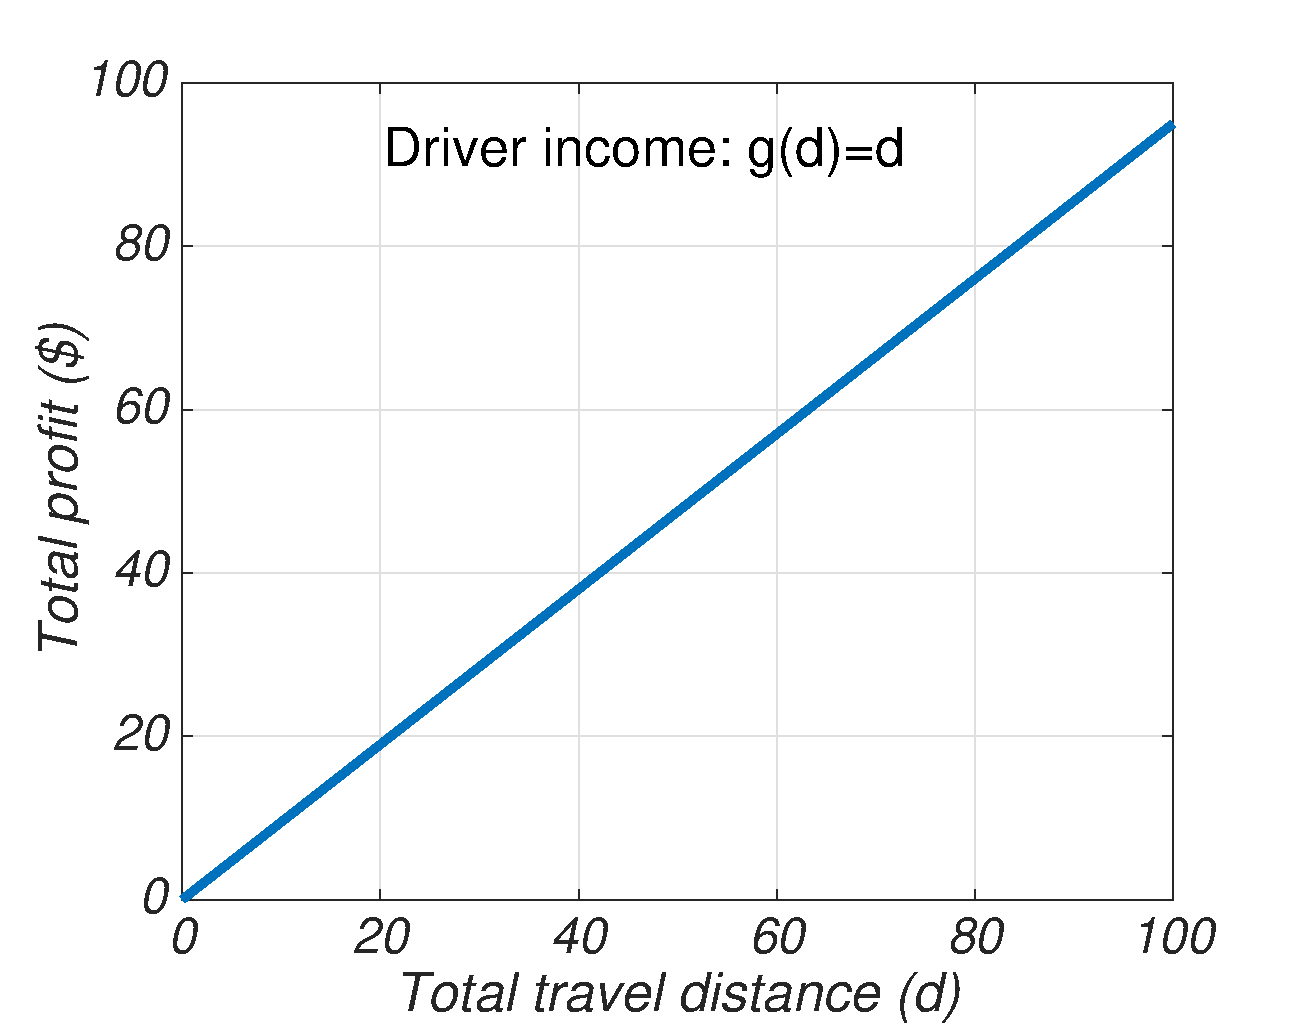
\includegraphics[width = 60mm]{fig/driver.eps}
	\vspace{-0mm}\caption{Driver profile} \vspace{-2mm} \label{fig:driver_profile}
\end{figure}\vspace{-0mm}
 
At any point in time, each driver has a schedule. A driver will be compensated during the time its schedule is not empty. Therefore, for every driver $v$, the income is:

\begin{equation}
\label{eq:payment}
income_v = \int_{start_s}^{end_s} I\left( s_v(t) \neq \left\langle \right\rangle\right).g(dist(t))dt
\end{equation}

\noindent Where $I()$ is the indicator function, $s_v(t)$ and $dist(t)$ are the driver's schedule and the distance he travels at time $t$ respectively. In addition, $start_s$ and $end_s$ are the first pick-up time and last drop-off time of $s_v$. Consequently, regardless of the serviced requests, each driver receives an income only based on his total traveled distance which satisfies the second rule of a fair pricing model.

\subsection{Revenue}

What the driver makes does not necessarily have to be the same as what the riders pay (i.e., the $FARE$ method) for the same distance. It is the job of the framework to assign riders with drivers where their profiles are compatible (\TODO{mohammad}{use a similar thing in the intro and define what it means for profiles to be compatible}. By assigning riders to drivers such that the fare riders pay is more than what the drivers make without violating anyone's monetary incentive, APART can add to its profit. The profit APART makes from driver $v$ is the difference between the fares collected from all riders serviced by $v$ and the income $v$ receives for himself. Subsequently, the total profit (revenue) of APART is be the sum of the profits received from all drivers:

\begin{align}
\label{eq:profit} 
profit_v &= \sum_{r_i \in s_v}fare(r_i) - cost_v\\
revenue &= \sum_{v \in V}profit_v
\end{align}
